\section{Auswertung}
\label{sec:Auswertung}
\subsection{Ermittelung der mittleren freien Weglänge}
Die mittlere freie Weglänge der Elektronen kann mithilfe von 
Formel (\ref{eqn:Sättigungsdampfdruck}) und (\ref{eqn:mittlereWeglängeAtome}) 
berechnet werden. Die dazu verwendeten 
Temperaturen $T$, bei denen die Kurven aufgenommen werden, 
sind in Tabelle (\ref{tab:Weglaenge}) zusammen mit den Ergbenissen 
aufgelistet. Außerdem wird das Verhältnis aus dem Abstand 
$a = 1 \, \unit{\centi\meter}$ zwischen Kathode und 
Elektrode und der mittleren freien Weglänge berechnet 
und in Tabelle (\ref{tab:Weglaenge}) aufgelistet.           
\begin{table}[H]
    \centering
    \caption{Mittlere freie Weglänge mit Verhältnis}
    \label{tab:Weglaenge}
    \begin{tblr}{colspec={c c c}}
        \toprule
        $\text{T} \left[\unit{\kelvin}\right]$ & $\bar{\omega} \left[\unit{\meter}\right]$ & $a/ \bar{\omega}$\\
        \midrule  
        $295,75$ & $6,59 \cdot 10^{-3}$ & $1,52$\\ 
        $423,15$ & $6,01 \cdot 10^{-6}$ & $1,66 \cdot 10^{3}$\\ 
        $433,15$ & $4,13 \cdot 10^{-6}$ & $2,42 \cdot 10^{3}$\\ 
        $444,15$ & $2,79 \cdot 10^{-6}$ & $3,59 \cdot 10^{3}$\\ 
        $451,15$ & $2,19 \cdot 10^{-6}$ & $4,56 \cdot 10^{3}$\\ 
        $453,15$ & $2,05 \cdot 10^{-6}$ & $4,88 \cdot 10^{3}$\\
        \bottomrule
    \end{tblr}
\end{table}
Das Verhältnis nimmt mit steigender Temperatur zu. 
\subsection{Differentielle Energieverteilung}
Die zugrundeliegende Messkurve wird mithilfe eines 
x-y-Schreibers aufgezeichnet. Die Messkurve, die bei einer 
Temperatur von $22,6 \, °\text{C}$ aufgenommen wird, ist 
in Abbildung (\ref{fig:22,6}) zu sehen. Die Messkurve, die bei 
$150 \, °\text{C}$ aufgenommen wird, ist in Abbildung 
(\ref{fig:150}) zu sehen. Beide Kurven werden bei einer
Beschleunigungsspannung von $U_B = 11 \, \unit{\volt}$
aufgenommen. 
\begin{figure}
    \centering
    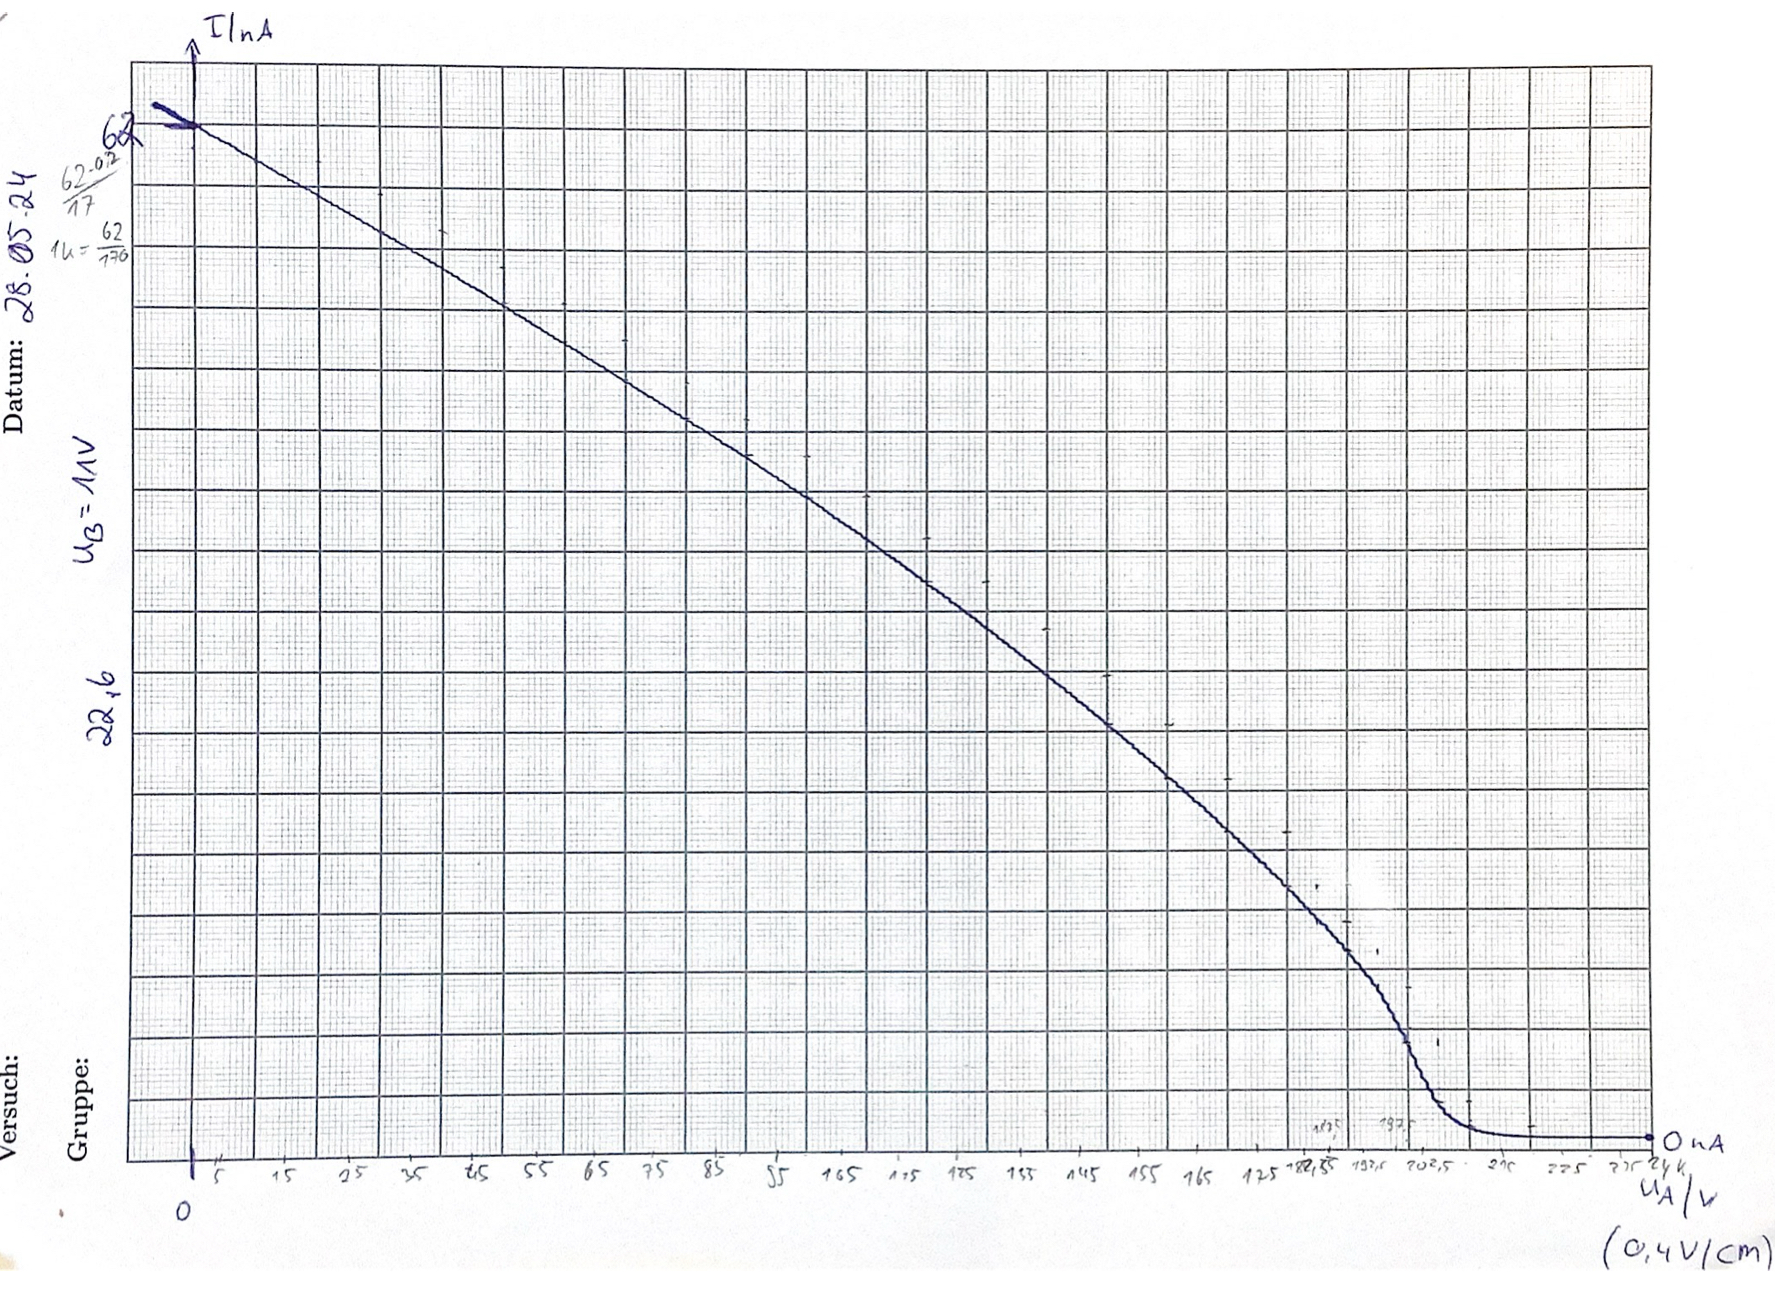
\includegraphics[width=0.8\textwidth]{content/Bilder/22,6.jpeg}
    \caption{Strom-Spannungsmesskurve bei T = 22,6 °C.}
    \label{fig:22,6}
\end{figure}
\begin{figure}
    \centering
    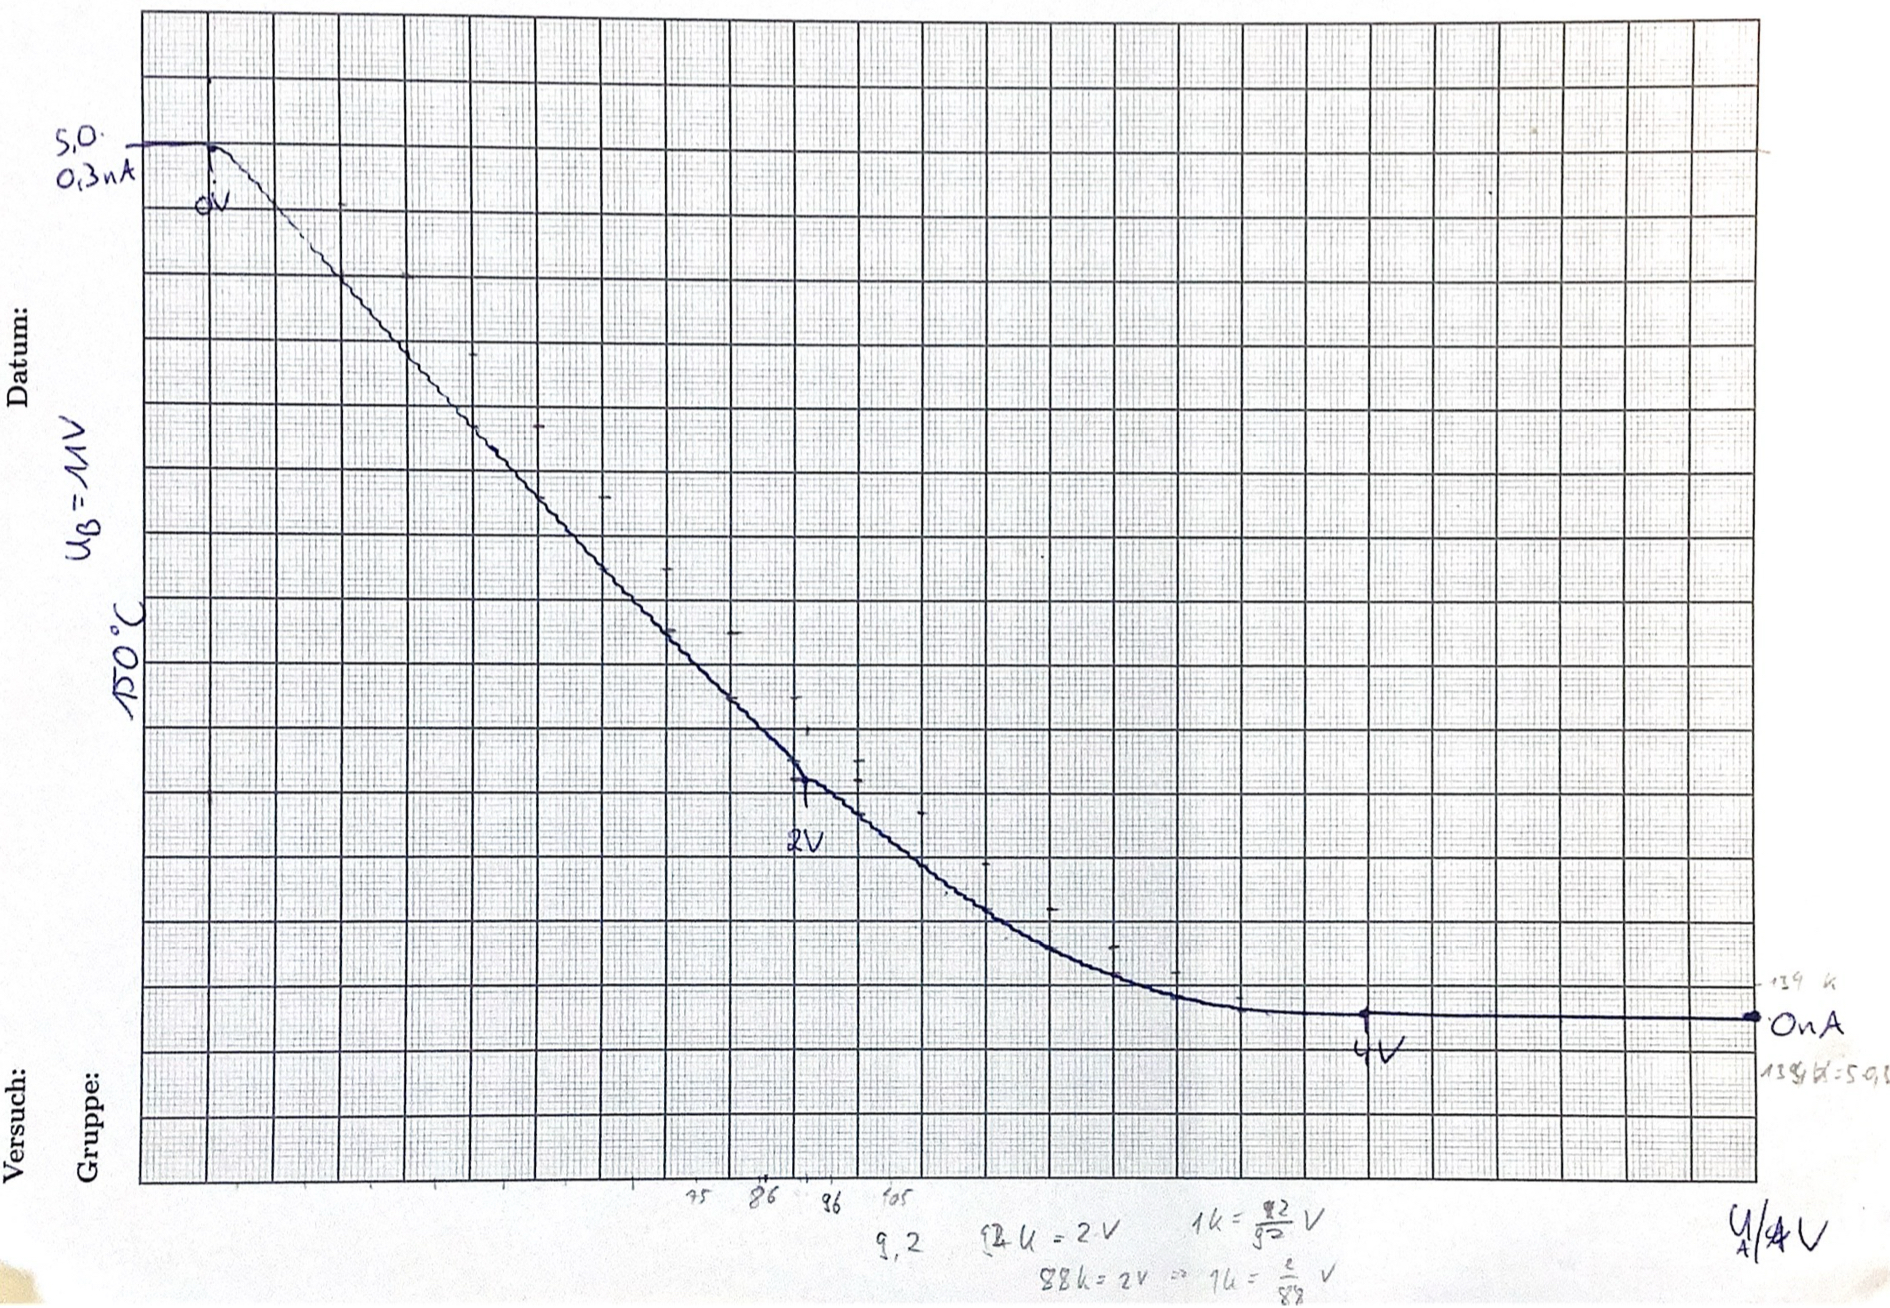
\includegraphics[width=0.8\textwidth]{content/Bilder/150.jpeg}
    \caption{Strom-Spannungsmesskurve bei T = 150 °C.}
    \label{fig:150}
\end{figure}

\subsection{Franck-Hertz-Kurve und Anregungsenergie}
% \begin{figure}
%   \centering
%   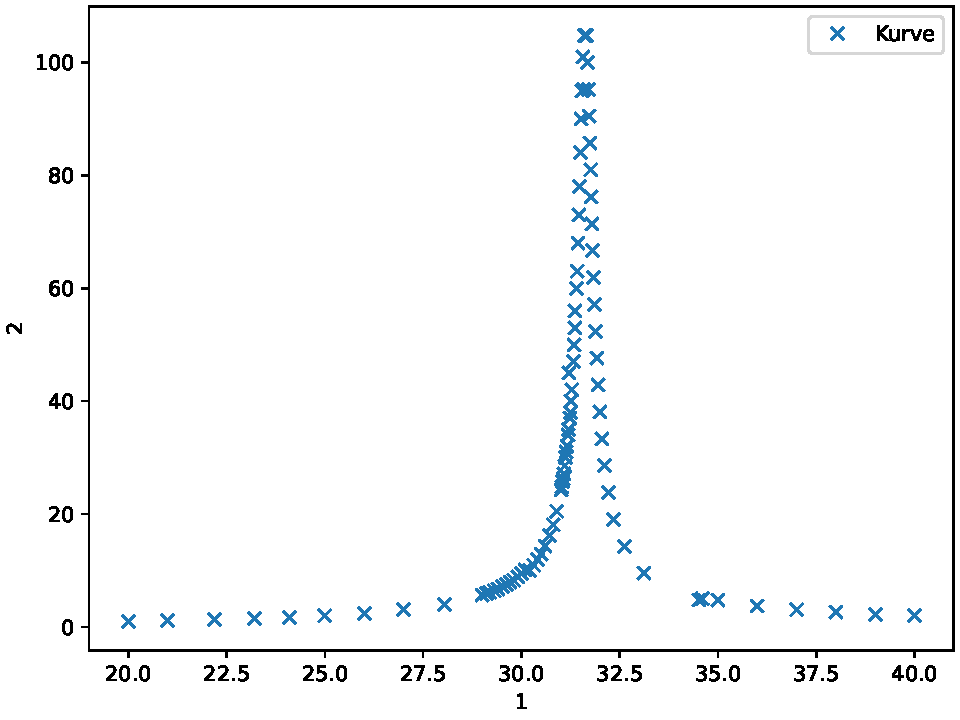
\includegraphics{plot.pdf}
%   \caption{Plot.}
%   \label{fig:plot}
% \end{figure}

%Siehe \autoref{fig:plot}!